\documentclass[12pt,english,dvipsnames,aspectratio=169, handout]{beamer}
\usepackage{fontspec}
\setsansfont[Mapping=tex-text]{Fira Sans}
\setcounter{secnumdepth}{4}
\setcounter{tocdepth}{4}
\usepackage[normalem]{ulem}
\usepackage[T1]{fontenc}
\usepackage{dcolumn}
\usepackage{booktabs}
\usepackage{setspace}
\makeatletter
\usetheme{metropolis}
\setbeamertemplate{frame footer}{Bosancianu | Schaub | Hertie School}
\setbeamerfont{page number in head/foot}{size=\tiny}
\setbeamercolor{footline}{fg=gray}
\usepackage{xcolor}
\usepackage{tikz}
\usepackage[labelformat=empty]{caption}
% For table captions in Beamer
\usepackage[sectionbib]{apacite}
\renewcommand{\bibliographytypesize}{\footnotesize}
\makeatletter
\let\st@rtbibsection\@bibnewpage
\let\st@rtbibchapter\@bibnewpage
\makeatother
\usepackage{amsmath, mathtools}
\usepackage{xunicode}
\usepackage{hyperref}
\graphicspath{{./figures/}} 
% Defines a checkmark
\def\checkmark{\tikz\fill[scale=0.4,color=orange](0,.35) -- (.25,0) -- (1,.7) -- (.25,.15) -- cycle;}
\setbeamertemplate{itemize items}{\checkmark}
\usepackage{multirow}
\hypersetup{pdfauthor={Bosancianu and Schaub},
	pdftitle={Statistical Modeling and Causal Inference with R},
	pdfsubject={Week 1: Introduction},
	pdfkeywords={Berlin, Hertie, 2020, week 1}}
\title{\textsc{Statistical Modeling and Causal Inference with R}}
\subtitle{Week 1: Introduction}
\date{September 7, 2020}
\author{Manuel Bosancianu \hfill Max Schaub}
\institute{Hertie School of Governance}
\begin{document}
\maketitle

\begin{frame}
	\frametitle{Today's focus}
	
	\begin{itemize}
		\setlength\itemsep{1.5em}
		\item Welcome and introductions
		\item Course logistics
		\item Why study causal inference?
	\end{itemize}
\end{frame}


\section{Welcome}
\begin{frame}[plain]
	\begin{center}
		\Huge Thank \textcolor{orange}{you} for joining us in the course! 
	\end{center}
\end{frame}

\begin{frame}
	\frametitle{The team (I)}
	\begin{minipage}[t]{0.48\linewidth}
		\footnotesize
		\textbf{Manuel}
		\begin{itemize}
			\item Research fellow at the WZB Berlin Social Science Center
			\item Political Economy of Development
			\item Interests: political inequality, economic inequality, Leftist parties, data visualization
			\item Methods: multilevel modeling, Bayesian analysis, experimental (recent), causal inference
		\end{itemize}
	\end{minipage}\hfill
	\begin{minipage}[t]{0.48\linewidth}
		\footnotesize
		\textbf{Max}
		\begin{itemize}
			\item Research fellow at the WZB Berlin Social Science Center
			\item Migration and Diversity
			\item Interests: migration, violence, poverty, political participation
			\item Methods: causal inference, survey design, field and lab-in-the-field experiments
		\end{itemize}
	\end{minipage}
\end{frame}


\begin{frame}
	\frametitle{What's your profile?}
	
	How many\dots graduated a quantitative-focused program in economics, political science, etc?\bigskip

	\pause

	\dots are familiar with Stata (wrote the analysis for a paper with it)?\bigskip

	\pause

	\dots are familiar with R (had a class with it)?\bigskip
	
	\pause
	
	\dots can name the assumptions needed to make OLS a BLUE?
	
\end{frame}

\begin{frame}
	\frametitle{The course: goals}
	\begin{itemize}
		\setlength\itemsep{1.5em}
		\item To train your ability to look at research designs from a causal perspective
		\item To increase your discernment regarding the causal foundations of empirical analyses
		\item To provide you with a standard toolbox of approaches to causal inference
		\item To accustom you with how these are implemented in \texttt{R}
	\end{itemize}
		
\end{frame}


\begin{frame}
	\frametitle{The course: topics}
	\begin{enumerate}
		\item Potential outcomes framework \& Causal graphs
		\item IV estimation
		\item Matching
		\item Regression discontinuity designs
		\item Difference-in-Difference designs \& Synthetic controls
		\item Panel data \& Fixed Effects
		\item Moderation \& Mediation
		\item Field experiments
	\end{enumerate}

\begin{center}
	A ``fox'', rather than a ``hedgehog'' (Sir Isaiah Berlin).
\end{center}
	
\end{frame}


\begin{frame}
	\frametitle{The course: readings}
	Three tiers:
	
	\begin{enumerate}
		\setlength\itemsep{1em}
		\item \textbf{required}: copies of \textit{Mastering 'Metrics} have been bought and put on reserve by the library
		\item \textbf{optional}: if you're particularly interested in the topic
		\item \textbf{applied}: practical example for method (focus only on underlined one in syllabus)
	\end{enumerate}
	
	All required readings, and one of the applied ones, are to be done before Monday's sessions.
	
\end{frame}


\section{Logistics}
\begin{frame}
	\frametitle{The class setting}
	You will have lectures in video format available on Friday the week before our Monday meeting.\bigskip
	
	In class, we hope you will be the stronger force in pushing the discussion:
	
	\begin{itemize}
		\item If readings or video lecture weren't clear, please ask questions!
		\item If tempo is too rapid (or slow), please let us know!
	\end{itemize}

    Many opportunities to re-visit material: Monday sessions \& initial part of labs.
	
\end{frame}


\begin{frame}
	\frametitle{Attendance}
	You've been allocated to 3 groups, and switching is generally \textbf{not possible}. Let us know in advance if you cannot join your group, and want to switch.\bigskip
	
	12 sessions in total, meaning \textbf{you cannot skip more than 2}.\bigskip
	
	If you cannot make it at all (e.g. health reasons, personal emergencies), please let the Examination Office know beforehand---they will inform us.\bigskip
	
	We have to take attendance, partly for public health reasons.
	
\end{frame}


\begin{frame}
	\frametitle{Other points of contact}
	Labs (drop-in) sessions are not mandatory, but highly encouraged---lots of \texttt{R} practice.\bigskip
	
	Labs also allow one more opportunity to ask questions about lecture material.\bigskip
	
	Finally, we offer office hours, via Zoom or Teams video call:
	
	\begin{itemize}
		\item Max: Thursdays, 14--16
		\item Manuel: Thursdays, 10--12
	\end{itemize}
	
	Please send us an email in advance with what you want to discuss (in case we need to prepare a bit beforehand).
	
\end{frame}


\begin{frame}
	\frametitle{Bi-weekly Assignments}
	Problem sets that combine conceptual and applied tasks.\bigskip
	
	Collaboration is encouraged while learning, but bi-weekly assignments are individual work.\bigskip
	
	\begin{table}
	\scriptsize
	\begin{tabular}{c c}
		\toprule
		\textbf{Assignment ``live''} & \textbf{Deadline} (always 11:59 PM CET) \\
		\midrule
		14.09 & 23.09 \\
		28.09 & 07.10 \\
		12.10 & 28.10 \\
		02.11 & 11.11 \\
		16.11 & 25.11 \\
		\bottomrule
	\end{tabular}
	\end{table}

\end{frame}


\begin{frame}
	\frametitle{Bi-weekly Assignments}
	Submit your answers via Moodle: (1) \texttt{.Rmd} file with answers, code, and output; (2) Knitted HTML file.\bigskip
	
	Final grade for this component is weighted average of 5 grades, with equal weights.\bigskip
	
	Each day of delay in submission results in a 10\% drop in the grade.
\end{frame}

\begin{frame}
	\frametitle{Additional assessments}
	
	\begin{table}
		\scriptsize
		\begin{tabular}{c c c c}
			\toprule
			\textbf{Type} & \textbf{Deadline} & \% of final grade \\
			\midrule
			Bi-weekly assignment & See above  & 40\% \\
			Final exam & TBC & 25\%  \\
			Replication task & 22.12 11:59 PM CET & 35\%  \\
			\bottomrule
		\end{tabular}
	\end{table}

For all of these, submission is via the Moodle system.\bigskip

Final exam is an at-home 120-minute test with open-ended questions, multiple choice questions, model output interpretation, graphs, and very simple calculations.
	
\end{frame}

\begin{frame}
	\frametitle{Additional assessments}
	Replication task based on set of recent published articles.\bigskip
	
	The challenge is to replicate the analyses in the article, and go beyond them, by exploring additional questions.\bigskip
	
	Final submission in paper (6--8 pages) and \texttt{Rmd} file. Short, but time consuming!
	
\end{frame}


\begin{frame}
	\frametitle{Labs (drop-in sessions)}
	Run entirely by \textbf{Adelaida Barrera} and \textbf{Sebastian Ramirez Ruiz}.\bigskip
	
	Voluntary attendance, but encouraged:
	
	\begin{itemize}
		\item Covering lecture content, if need be;
		\item Going over tasks similar to what assignments will cover
		\item Additional \textsf{R} practice
	\end{itemize}
	
\end{frame}


\section{Health considerations}
\begin{frame}
	\frametitle{In-person teaching}
	Participants are asked to wear masks when moving to and from desks. Masks can be taken off at the desk.\bigskip
	
	Instructors will teach without mask, from fixed position.\bigskip
	
	Minimum: 1.5 meters (without mask), 1 meter (with mask).\bigskip
	
	If you have any concerns about this policy, please let us know early, so we can address them.\bigskip
	
	Attendance sheets will be used by Berlin health authorities to track movement, in case of infection.
	
\end{frame}


\begin{frame}
	\frametitle{Room use}
	Airing to take place at least once every 30 minutes.\bigskip
	
	Disinfectant spray and paper towels are available for use.\bigskip
	
	In case of any Covid-19-like symptoms, please don't come to class, and immediately notify Student Life office and Berlin health authorities (see Hertie \textbf{Hygiene Policy, v2}).\bigskip
	
	Instructors are subject to same rules in case of symptoms.
	
\end{frame}



\begin{frame}[plain]
	\begin{center}
		\Huge Chance to ask questions before we move to \textcolor{orange}{causality}\dots 
	\end{center}
\end{frame}

%%% Max
\section{Why study causal inference?}

\begin{frame}
	\frametitle{Why study causal inference?}
	\begin{enumerate}
		\setlength\itemsep{1.5em}
		\item Overcoming flaws in traditional statistical methods
		\item A new way of thinking about the world
		\item Answer questions we care about -- in a rigorous way
	\end{enumerate}
	
\end{frame}


\begin{frame}{Questions we care about\ldots}
\begin{itemize}
	\item Does micro-finance \textbf{affect} individuals' poverty status?
	\item Can personal experiences of extreme weather \textbf{shift} people's perception of climate change?
	\item Can we \textbf{demonstrate} that policing is racially biased?
	\item Can technological innovations \textbf{improve} political accountability and infant health?
\end{itemize}
``affect'', ``shift'', ``demonstrate'', ``improve'' all imply we are interested in \textbf{causal relationships}
\end{frame}

\begin{frame}{Overcoming flaws in traditional statistical methods}
The ladder of abstraction \cite{pearl_book_2018}
    \begin{figure}
    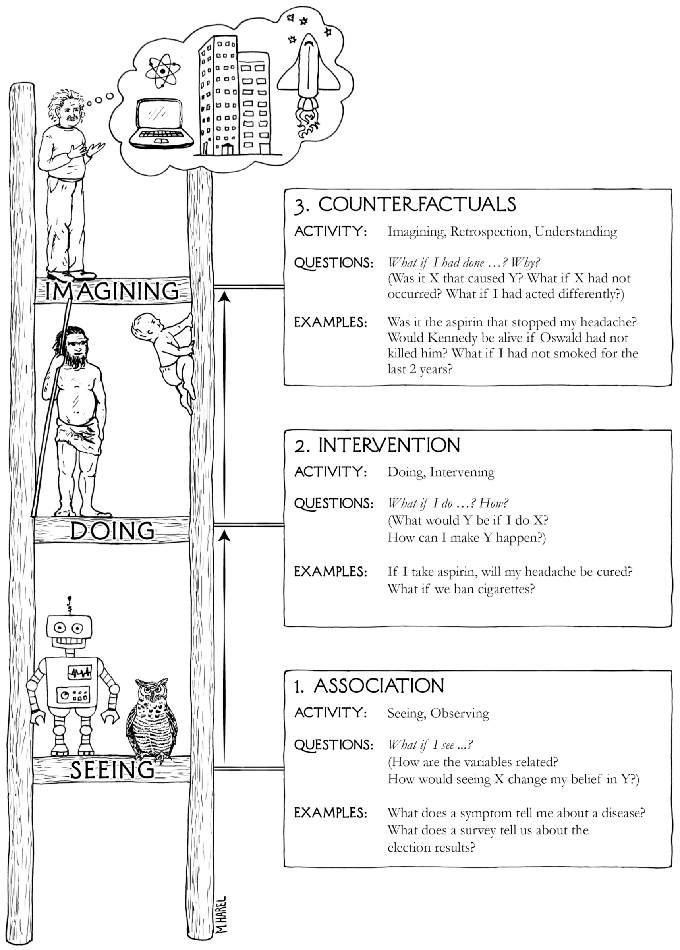
\includegraphics[height=.75\textheight]{../04-figures/01/01-Pearl2018Ladder}
    \end{figure}
\end{frame}


\begin{frame}{Overcoming flaws in traditional statistical methods}
\begin{itemize}
	\item Tailored towards `seeing' instead of `doing' \cite{pearl_book_2018}
	\item Non-directionality: $y = a + bx \xleftrightarrow{} x = (y-a)/b$		
	\item Threat of confounding by third variables -- and no guidance how to avoid it
	\item Lack of `shoe-leather'/ dominance of out-of-the-box solutions \cite{freedman_statistical_1991}
	\item ``Correlation is not causation''\\\ldots\textcolor{orange}{but what, then, is causation?}
\end{itemize}
\end{frame}

\begin{frame}{A new way of thinking about the world}
\textbf{Counterfactual thinking} and the potential outcomes framework 
    \begin{figure}
    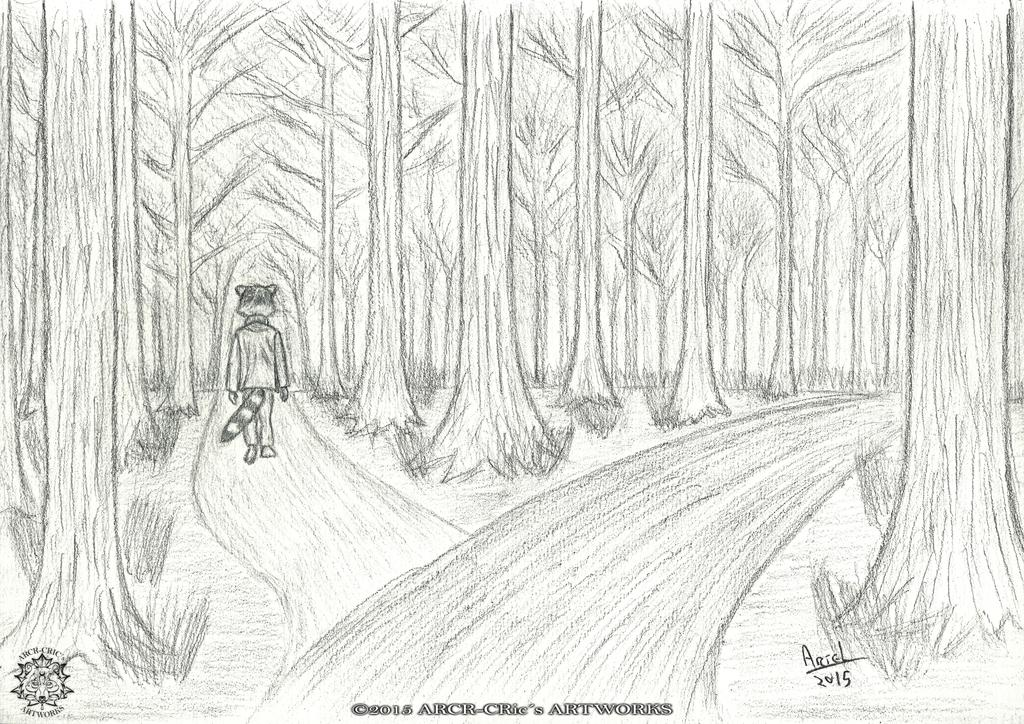
\includegraphics[width=.6\textwidth]{../04-figures/01/02-the_road_not_taken_by_arcr_cric}
    \end{figure}
\end{frame}


\begin{frame}{A new way of thinking about the world}
Counterfactual thinking and the \textbf{potential outcomes framework} 
	\begin{equation*}
	\text{Causal effect: } {\Delta_i = Y_{i1} - Y_{i0}}
	\end{equation*}
\end{frame}


\begin{frame}{Answer questions we care about -- in a rigorous way}
\textbf{Example}: Effect of micro-finance on poverty status
\begin{itemize}
	\item Imagine you were asked to assess the effect of receiving a micro-finance loan on income 5 years later?
	\item \textcolor{orange}{What would you do to find out?}
\end{itemize}
\end{frame}



\begin{frame}{Answer questions we care about -- in a rigorous way}
\textbf{Conduct experiments/ randomized control trial (RCTs)}
\begin{enumerate}
	\item Intervention (e.g.\ access to micro-finance)
	\item Randomly assign individuals to treatment and control
	\item Compare outcomes (taking into consideration treatment compliance issues)
\end{enumerate}
\end{frame}


\begin{frame}{Answer questions we care about -- in a rigorous way}
\textbf{Example (cont'd)}: Effect of micro-finance on poverty status 
\begin{itemize}
	\item Imagine you are given a dataset with data on individuals' incomes who received/did not receive loan
	\item Data shows that individuals who received a loan were doing better
	\item \textcolor{orange}{Can we conclude that micro-finance had a positive causal effect?}
\end{itemize}
\end{frame}

\begin{frame}{Answer questions we care about -- in a rigorous way}
\textbf{Analyze observational data in terms of hypothetical experiments \cite{rubin_objective_2008}}
\begin{enumerate}
	\item What would the ideal experiment have looked like?
	\item What was the process of treatment assignment, and how did it deviate from random?
	\item Account for these deviations (if at all possible), and compare outcomes
\end{enumerate}
\end{frame}

\begin{frame}{Answer questions we care about -- in a rigorous way}
\textbf{Use causal diagrams/directed acyclic graphs (DAGs) \cite{pearl_book_2018}}
    \begin{figure}
    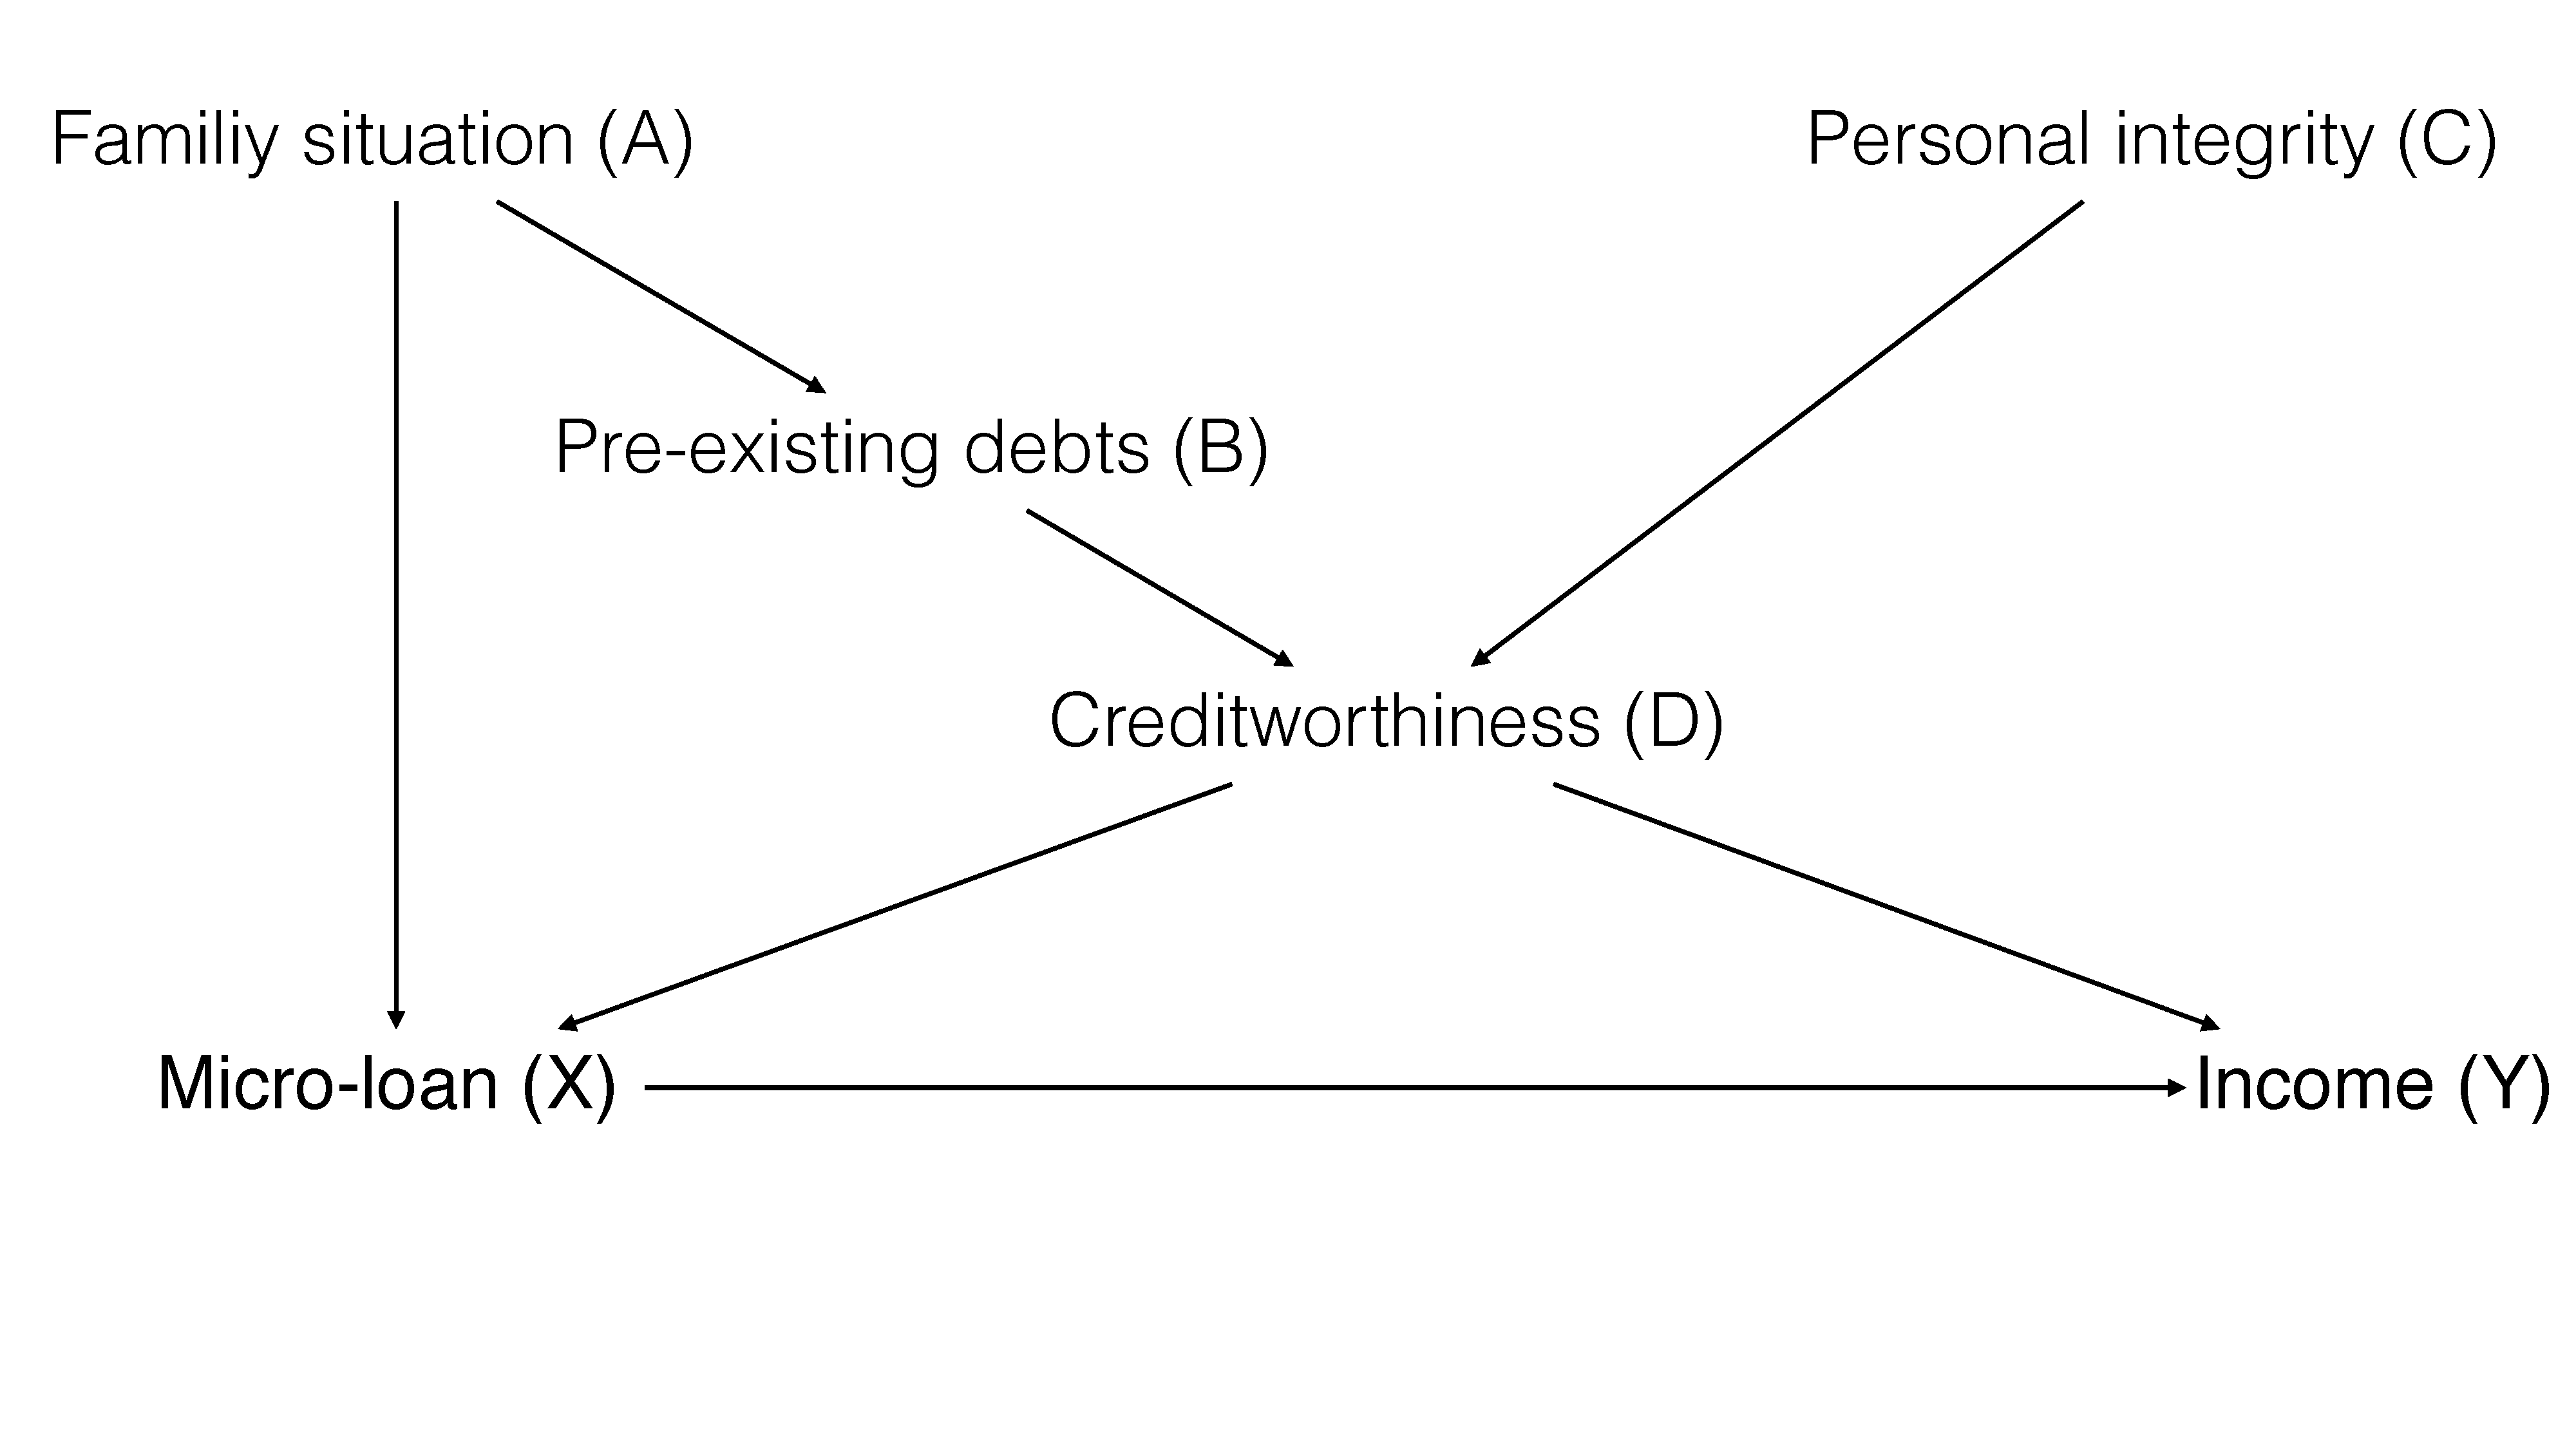
\includegraphics[width=.8\textwidth]{../04-figures/01/03-dag_micfin}
    \end{figure}
\end{frame}

\begin{frame}{Answer questions we care about -- in a rigorous way}
\textbf{Use causal diagrams/directed acyclic graphs (DAGs) \cite{pearl_book_2018} -- and try to shut backdoors to potential confounders}
    \begin{figure}
    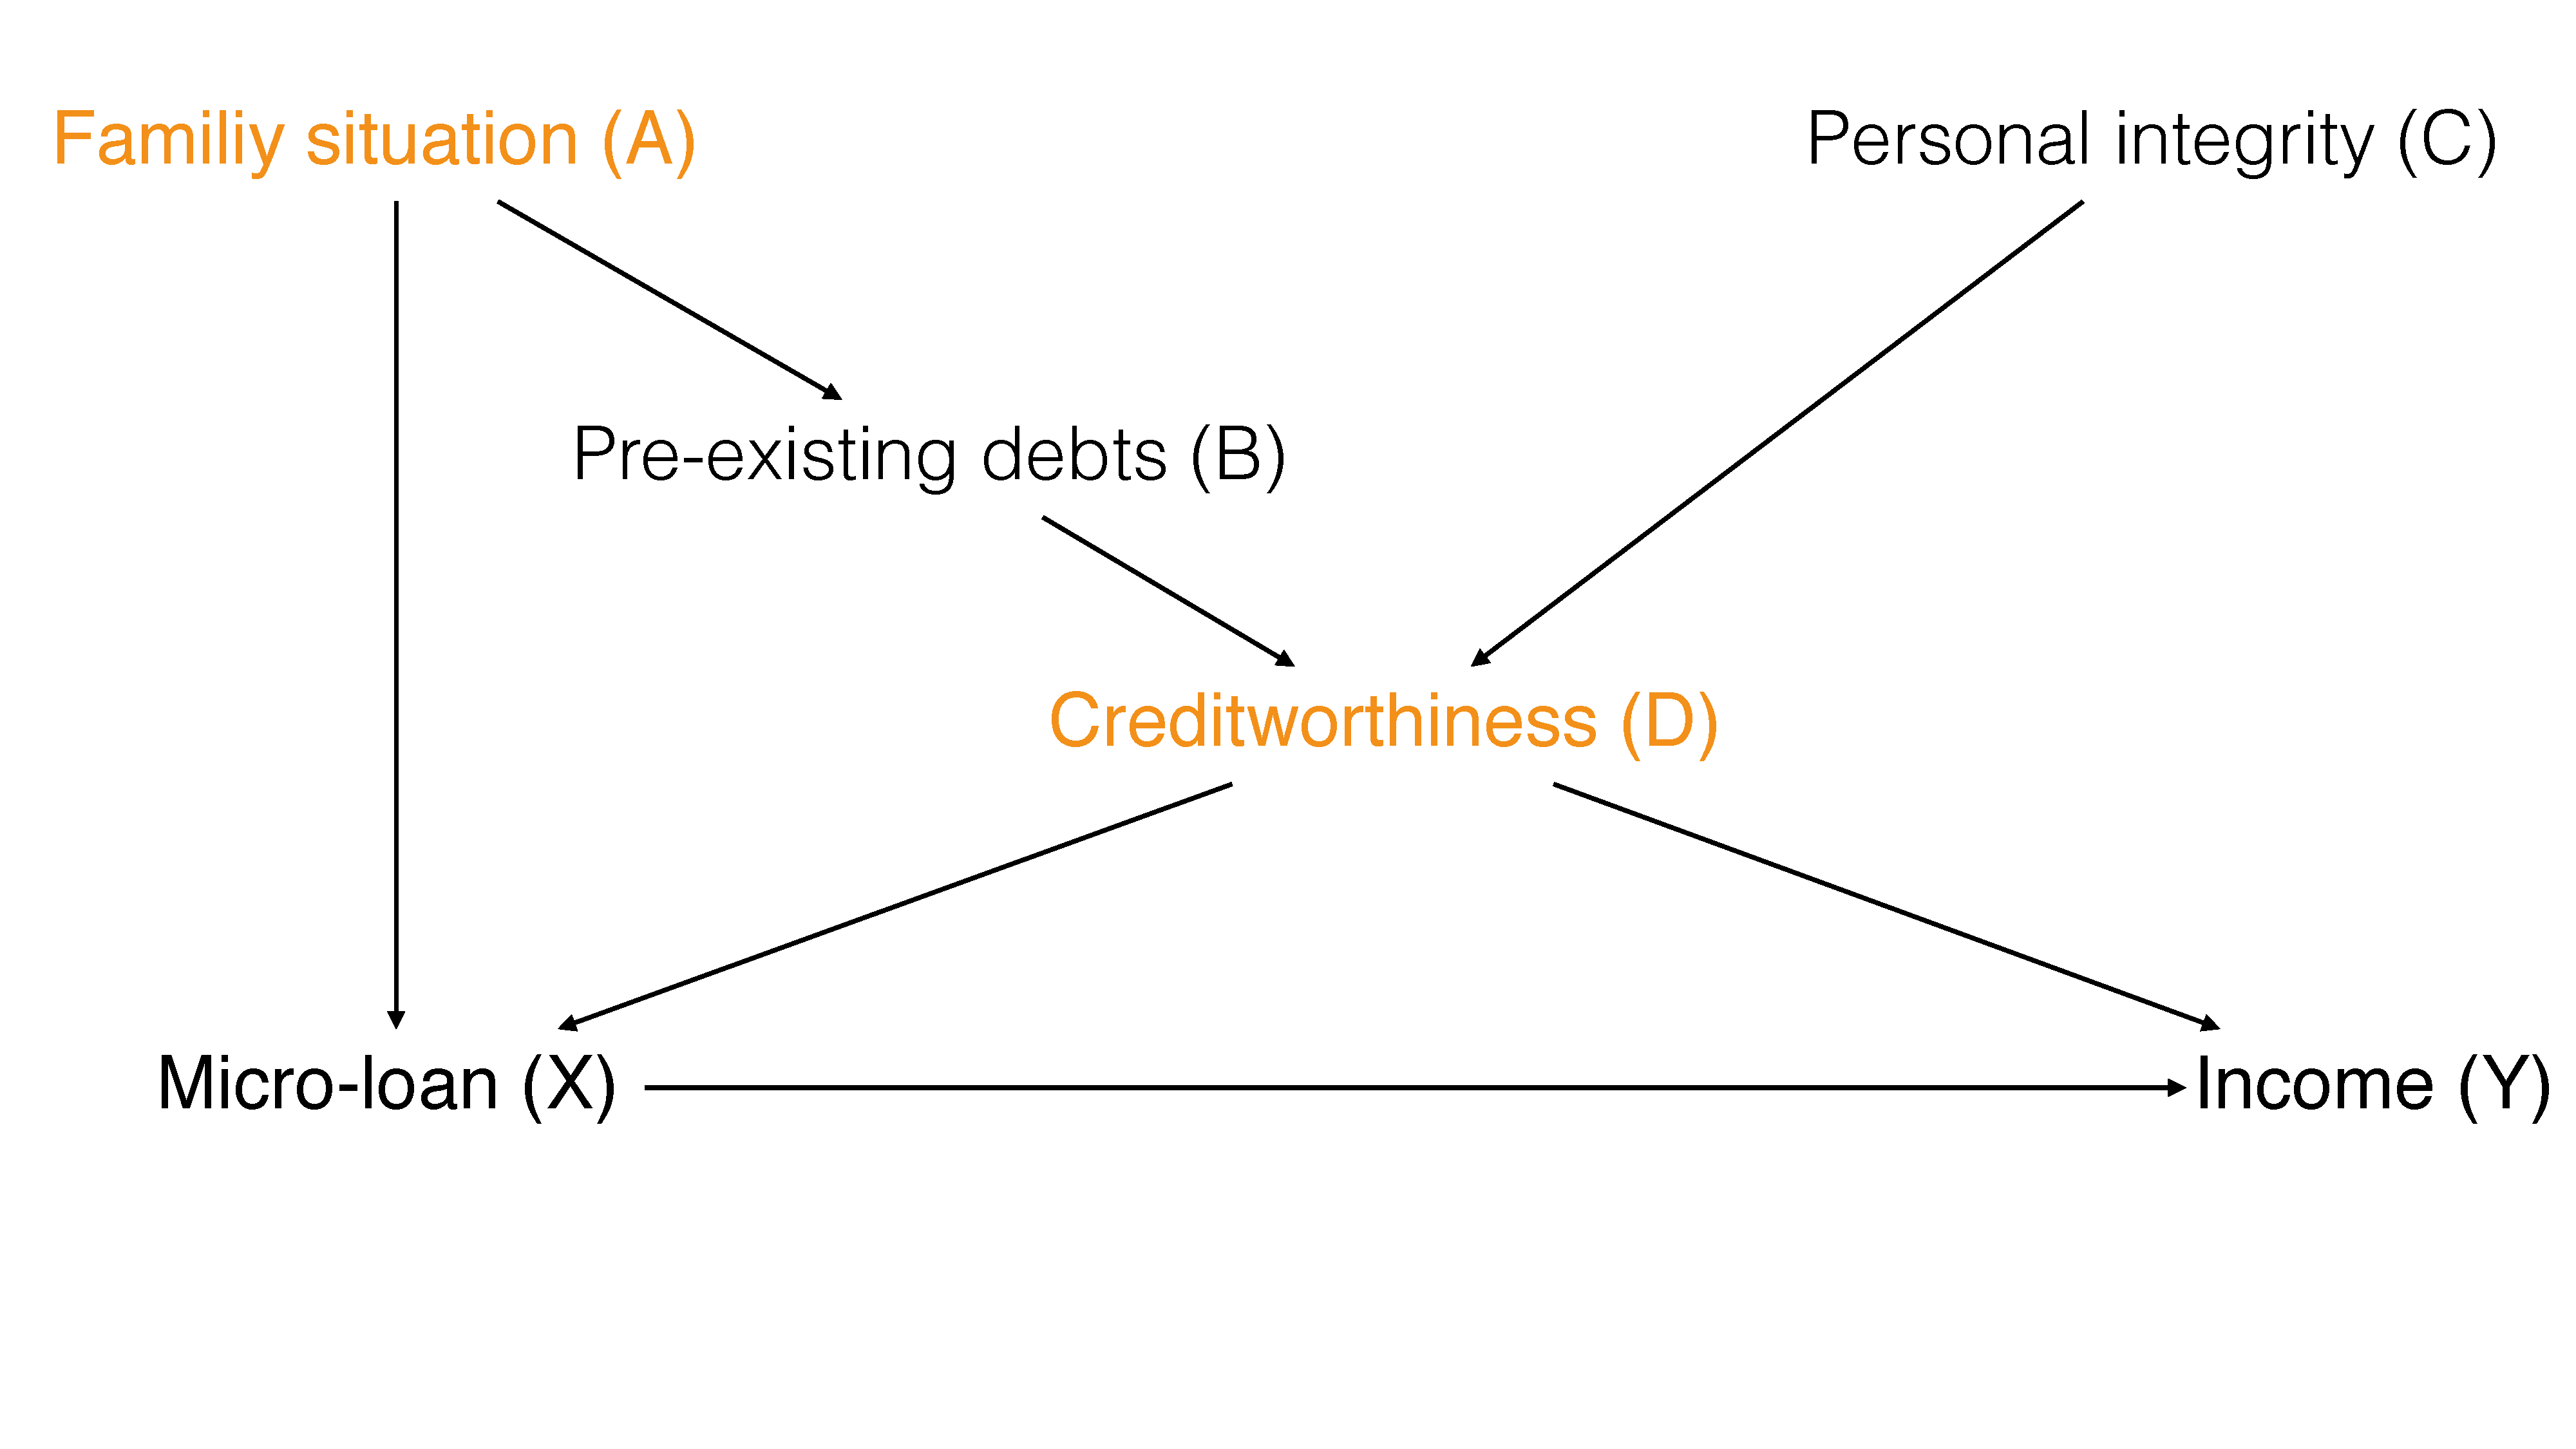
\includegraphics[width=.8\textwidth]{../04-figures/01/04-dag_micfin_c}
    \end{figure}
\end{frame}


% END
\begin{frame}
\begin{center}
    \Huge Thank \textcolor{orange}{you} for the kind attention!
\end{center}
\end{frame}

% REFERENCES %

\begin{frame}
\frametitle{References}
\bibliographystyle{apacite}
\bibliography{../Bibliography}
\vspace{5cm}
\end{frame}

\begin{frame}{Answer questions we care about -- in a rigorous way}
\textbf{Conduct experiments/ randomized control trial (RCTs): \emph{do} micro-loan}
    \begin{figure}
    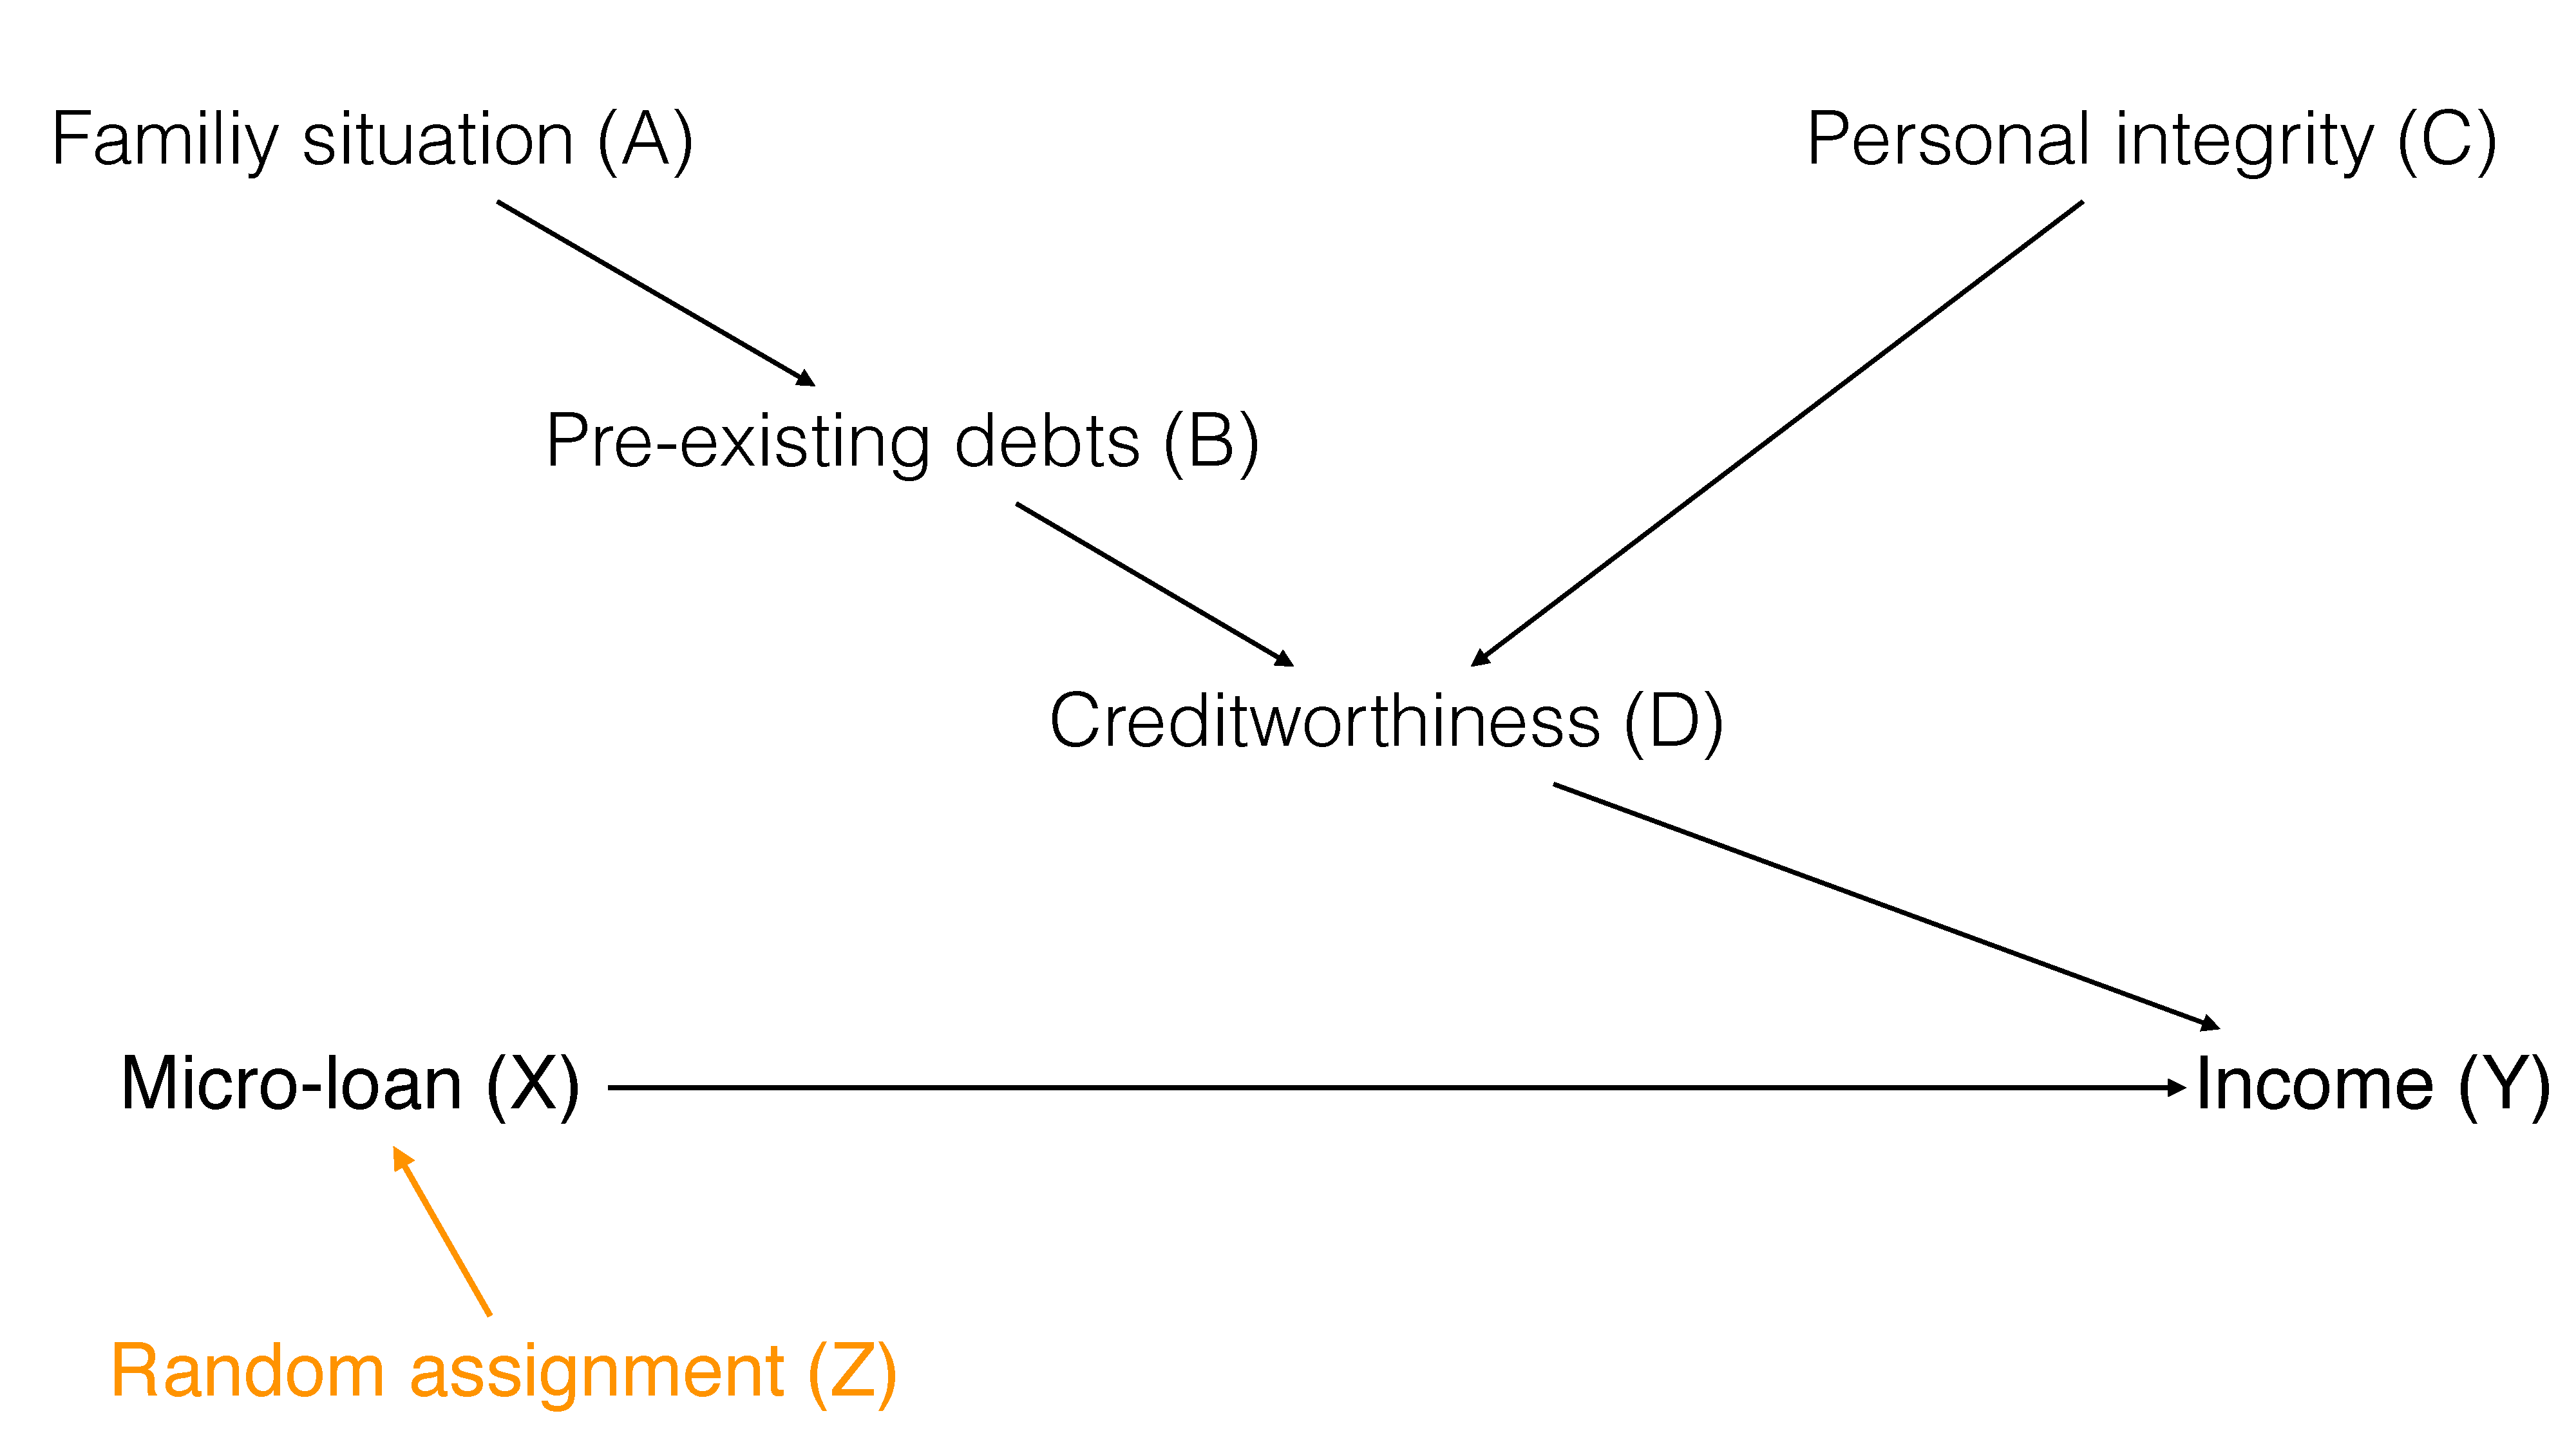
\includegraphics[width=.8\textwidth]{../04-figures/01/05-dag_micfin_r}
    \end{figure}
\end{frame}

\end{document}